\documentclass[12pt,t]{beamer}
\usepackage{graphicx}
\usepackage[vlined]{algorithm2e}
\usepackage{times}
\usepackage{calc}
\usepackage{url}
\usepackage{soul}
\usepackage{graphicx}
\usepackage{multirow, hhline}
\usepackage{array, booktabs, colortbl}
\usepackage{amsmath}
\usepackage{amssymb}
\usepackage{relsize}
\usepackage{multirow}
\usepackage{booktabs}
\usepackage{pagecolor}
\usepackage{lipsum}
\usepackage{capt-of}
\usepackage{booktabs}

\usepackage{graphicx}
\usepackage{multicol}
\usepackage[T1]{fontenc}
\usepackage{ae}
\graphicspath{{fig/}}
\setbeameroption{hide notes}
\setbeamertemplate{note page}[plain]

\usetheme{default}
\beamertemplatenavigationsymbolsempty
\hypersetup{pdfpagemode=UseNone}

\usefonttheme{professionalfonts}
\usefonttheme{serif}
\usepackage{fontspec}
\setmainfont{Karla}
\setbeamerfont{note page}{family*=pplx,size=\footnotesize} % Palatino for notes

\definecolor{foreground}{RGB}{70,70,70}
\definecolor{background}{RGB}{249, 249, 249} %24,24,24
%\definecolor{title}{RGB}{107,174,214} %107,174,214
\definecolor{title}{RGB}{70,70,70}
\definecolor{gray}{RGB}{0,0,0}
\definecolor{subtitle}{RGB}{70,70,70}
\definecolor{hilight}{RGB}{102,255,204}
\definecolor{vhilight}{RGB}{255,111,207}
\definecolor{Gray}{gray}{0.85}
\definecolor{LiteGray}{gray}{0.92}

\setbeamercolor{titlelike}{fg=title}
\setbeamercolor{subtitle}{fg=subtitle}
\setbeamercolor{institute}{fg=gray}
\setbeamercolor{normal text}{fg=foreground,bg=background}


\setbeamercolor{item}{fg=foreground} % color of bullets
\setbeamercolor{subitem}{fg=gray}
\setbeamercolor{itemize/enumerate subbody}{fg=gray}
\setbeamertemplate{itemize subitem}{{\textendash}}
\setbeamerfont{itemize/enumerate subbody}{size=\footnotesize}
\setbeamerfont{itemize/enumerate subitem}{size=\footnotesize}

\setbeamercolor{block title}{fg=white,bg=gray!70}
\setbeamercolor{block body}{fg=black,bg=gray!10}
\setbeamercolor{block title alerted}{fg=red,bg=gray!40}
\setbeamercolor{block title example}{fg=black,bg=green!20}
\setbeamercolor{block body example}{fg=black,bg=green!5}
\setbeamerfont{block title}{series=\bfseries}

\hypersetup{colorlinks,linkcolor=foreground,urlcolor=foreground}


\setbeamertemplate{footline}{%
    \raisebox{5pt}{\makebox[\paperwidth]{\hfill\makebox[20pt]{\color{gray}
          \scriptsize\insertframenumber}}}\hspace*{5pt}}

\addtobeamertemplate{note page}{\setlength{\parskip}{12pt}}


\newcommand{\bi}{\begin{itemize}}
\newcommand{\ei}{\end{itemize}}
\newcommand{\ig}{\includegraphics}
\newcommand{\subt}[1]{{\footnotesize \color{subtitle} {#1}}}

\let\emph\relax % there's no \RedeclareTextFontCommand
\DeclareTextFontCommand{\emph}{\bfseries\em}

\def\imagetop#1{\vtop{\null\hbox{#1}}}

\setbeamertemplate{frametitle}
{\vskip4pt
  \leavevmode
%\hbox{%
\begin{beamercolorbox}[wd=\paperwidth,ht=2ex,dp=0ex]{frametitle}%
\underline{\makebox[\paperwidth][l]{\hspace*{10pt}
\large {{\insertframetitle}}}}
\end{beamercolorbox}
%  }%
}

%\setbeamercolor{frametitle}{fg=yellow,bg=red}

\begin{document}

\AtBeginSection[]{
  \begin{frame}
  \vfill
  \centering
  \begin{beamercolorbox}[sep=8pt,center,shadow=true,rounded=true]{title}
    \underline{\makebox[0.8\paperwidth][l]{
\large {{\insertsectionhead}}}}
  \end{beamercolorbox}
  \vfill
  \end{frame}
}

\title{\large{Workshop \#3: More on Regression Models}}
\subtitle{TRiCAM 2017}
\author{W. Pan}
%\institute{Harvard University}
\date{}
\titlegraphic{
   
\includegraphics[height=2cm]{iacs}
\includegraphics[height=2cm]{harvard}
\includegraphics[height=2cm]{hogwarts}
}
{
\setbeamertemplate{footline}{} % no page number here
\frame{
  \titlepage
  
}
}

\begin{frame}{Lecture Outline}
\tableofcontents
\end{frame}

%%%%%%%%%%%%%%%%%%%%%%%%%%%%%%%%%%%%%%%%%%%%%%%%%%%%%%%%%%%%%%%%%%%%%%%%%%%%%%
\section{Review: Statistical Regression Models}

\begin{frame}{Statistical Models: Summary} 
\vskip-0.4cm
Recall that a statistical model for an observation $y$, called the \emph{response variable}, based on \emph{predictor variables} $x_1, \ldots, x_J$, posits that:
\begin{enumerate}
\item a general mathematical relationship, $f(x_1, \ldots, x_J)$, between $y$ and $x_1, \ldots, x_J$,
\item the observed values of $y$ differ from $f(x_1, \ldots, x_J)$ by \emph{random noise}.
\end{enumerate}
That is, a statistical model for $y$ using the predictors $x_1, \ldots, x_J$ is
\[
y = f(x_1, \ldots, x_J) + \epsilon,
\]
where $\epsilon$ is a \emph{random variable}. 
\vskip0.2cm
In \emph{inference}, we fine the parameters of $f$ that minimizes a choice of \emph{loss function}. Learning the parameters of the function $f$ is called \emph{`fitting the model'}. 
\end{frame}

\begin{frame}{Simple Linear Regression}
\vskip-0.4cm
A \emph{simple linear regression} model is a statistical model where $f$ is a linear function
\[
y = a_1\cdot x + a_0 + \epsilon.
\]
Suppose that $\epsilon \sim \mathcal{N}(0, \sigma^2)$, then 
\[
y | a_1, a_0, x, \epsilon \sim \mathcal{N}(a_1\cdot x + a_0, \sigma^2).
\]
The normal pdf $p(y | a_1, a_0, x)$ is called the \emph{likelihood function}, and measures how likely the observed data is under the model $a_1\cdot x + a_0$.
\vskip0.2cm
For multiple observations, $\{(x_1, y_1), \ldots, (x_n, y_n) \}$, the likelihood function is 
\[
\mathcal{L}(a_1, a_0) =  \prod_{i=1}^n p(y_i | a_1, a_0, x_i) = \prod_{i=1}^n \mathcal{N}(y_i; a_1\cdot x_i + a_0, \sigma^2) .
\]
\end{frame}

\begin{frame}{Maximum Likelihood Estimate Model}
\vskip-0.4cm
Given a set of observations, $\{(x_1, y_1), \ldots, (x_n, y_n) \}$, there are good reasons to find $a^{MLE}_1$ and $a^{MLE}_0$ so that the likelihood function is maximized:
\[
a^{MLE}_1, a^{MLE}_0 = \underset{a_1, a_0}{\mathrm{argmax}}\; \mathcal{L}(a_1, a_0) = \prod_{i=1}^n p(y_i | a_1, a_0, x_i) .
\]
The parameters $a^{MLE}_1$ and $a^{MLE}_0$ are called \emph{maximum likelihood estimates}.
\vskip0.2cm
When $\epsilon \sim \mathcal{N}(0, \sigma^2)$, maximizing likelihood is equivalent to minimizing Mean Square Error (MSE)
\[
a^{MLE}_1, a^{MLE}_0 =  \underset{a_1, a_0}{\mathrm{argmin}}\sum_{i=1}^n \left| y_i - (a_1x_i + a_0)\right|^2 
\]
\end{frame}

\begin{frame}{Linear Regression in Multiple Variables}
\vskip-0.4cm
A \emph{multiple linear regression model} is a linear statistical model relating the response $y$ to multiple predictors $x_1, \ldots, x_J$:
\[
y = a_0 + a_1 x_1 + \ldots + x_Jx_J  + \epsilon.
\]
If we take $\epsilon\sim \mathcal{N}(0,\sigma^2)$, then $y | \text{model} $ is a normally distributed random variable, $y | \text{model} \sim \mathcal{N}(a_0 + a_1 x_1 + \ldots + x_Jx_J, \sigma^2)$. 
\vskip0.2cm
The MLE model parameters for observations $\{(x_{1,1}, \ldots, x_{1,J}), \ldots, (x_{n,1}, \ldots, x_{n,J}) \}$ are given by
\[
a^{MLE}_0, \ldots, a^{MLE}_J =  \underset{a_0, \ldots, a_J }{\mathrm{argmin}}\sum_{i=1}^n \left| y_i - (a_0 + a_1 x_{i, 1} + \ldots + x_Jx_{i, J})\right|^2 
\]
Fitting a \emph{multiple linear regression model} is same as finding the best fitting \emph{plane} for the data.
\end{frame}

\begin{frame}{Polynomial Regression}
\vskip-0.4cm
A \emph{polynomial regression model of degree $m$}, relating $y$ to a single predictor $x$, is the statistical model
\[
y = a_0 + a_1 x +a_2 x^2 + \ldots + a_mx^m  + \epsilon
\]
A polynomial model is secretly a multi-linear model with $m$ number of predictors, $\{ x, x^2, \ldots, x^m\}$. So, if $\epsilon\sim \mathcal{N}(0,\sigma^2)$, then 
\[
y | \text{model} \sim \mathcal{N}(a_0 + a_1 x +a_2 x^2 + \ldots + a_mx^m, \sigma^2)
\]
\vskip0.2cm
Polynomial regression models can also be applied to multiple predictors
\[
y = a_0 + (a_{1, 1} x_1 + \ldots + a_{m, 1}x_1^m) + \ldots + (a_{1, J} x_J + \ldots + a_{m, J}x_J^m )+ \epsilon.
\]
\end{frame}

%%%%%%%%%%%%%%%%%%%%%%%%%%%%%%%%%%%%%%%%%%%%%%%%%%%%%%%%%%%%%%%%%%%%%%%%%%%%%%
\section{Review: Evaluating Models}

\begin{frame}{MSE and $R^2$}
\vskip-0.4cm
For a set of observations 
\[
\{(x_{1,1}, \ldots, x_{1,J}, y_1), \ldots, (x_{n,1}, \ldots, x_{n,J}, y_n)\}
\]
we typically measure the `fitness'  of a model $\hat{y} = \hat{f}(x_{1,1}, \ldots, x_{1,J})$ we've learned by aggregating the prediction errors
\[
MSE = \sum_{i=1}^n \left| y_i - \hat{y}_i\right|^2 = \sum_{i=1}^n \left| y_i - \hat{f}(x_{1,1}, \ldots, x_{1,J})\right|^2
\]
Alternatively, we can also compute the \emph{explained variance}, the ratio of the variation of the model and the variation in the data. For $\epsilon \sim \mathcal{N}(0, \sigma^2)$, explained variance is
\[
0 \leq R^2 = 1 -  \frac{\sum_{i=1}^n \left| y_i -\overline{y}_i\right|^2}{\sum_{i=1}^n \left| \hat{y}_i -\overline{y}_i\right|^2} \leq 1
\]
\end{frame}

\begin{frame}{Train vs Test Error}
\vskip-0.4cm
By definition, our MLE model minimizes the MSE on the observed data. But the minimized MSE can still be very large (relatively) because the data is not linear or the observed data is skewed!
\vskip0.2cm
We need to also measure the fitness of our learned model on new data. To do this, we
\begin{enumerate}
\item split the data into a training set and a testing set prior to modeling
\item fit the model using training set; find the MSE and $R^2$, this is called \emph{training error}
\item use the fitted model to find the MSE and $R^2$ on the testing set, this is called \emph{testing error}
\end{enumerate}
\vskip0.2cm
Which type of error do you expect to be lower? Why?
\end{frame}

\begin{frame}{Bootstrapping and Standard Error}\small
\vskip-0.4cm
Typically, our datasets are larger than we can process all at once. We may choose to sample a smaller random set of observations from the data to fit our model.
\vskip0.2cm
But this means that our estimates will vary depending on the samples we draw! So just how `confident' can we be in our fitted model?
\vskip0.2cm
To gauge the variations of our fitted model depending on the sample data, we \emph{bootstrap}:
\vskip0.2cm
\begin{enumerate}
\item we sample multiple sets of observations, for each we fit a model
\item using our multiple fitted models, we compute the mean and variance of each estimated model parameter
\end{enumerate}
\vskip0.2cm
The variance of an estimated parameter is called its \emph{standard error}.
\end{frame}

\begin{frame}{Significance of Variables}
\vskip-0.4cm
Suppose your fitted linear model looks like:
\[
y = 1 + 2.1 x_1 + 10 x_2 + 0.001 x_3
\]
Which variable is more `important'? Why? Is your definition of `important' fair?
\vskip0.2cm
We can also gauge the \emph{statistical significance} of each estimated coefficient using \emph{p-values} (can be estimated using bootstrap). Smaller p-values indicate stronger evidence against that the variable is completely negligible. 
\vskip0.2cm
Analyzing the significance our estimated parameters after fitting the model is a necessary and standard step.
\end{frame}


%%%%%%%%%%%%%%%%%%%%%%%%%%%%%%%%%%%%%%%%%%%%%%%%%%%%%%%%%%%%%%%%%%%%%%%%%%%%%%
\section{Regularization and Bayesian Models}

\begin{frame}{Overfitting}
\vskip-0.4cm
\only<1-7>{One thing we notice immediately was that the error on the training set decreases as the degree of the polynomial increases. 
\vskip0.2cm
So maybe we generally want to pick very high degree polynomials to model our data?
\begin{center}
\only<1>{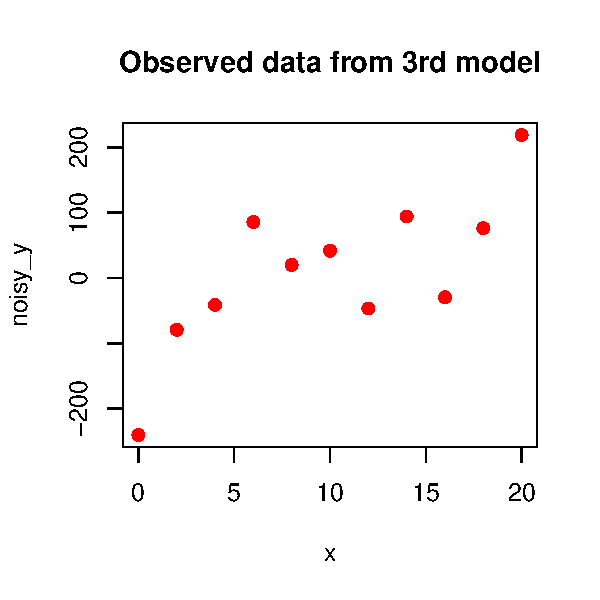
\includegraphics[height=35mm]{scatter_fit}}
\only<2>{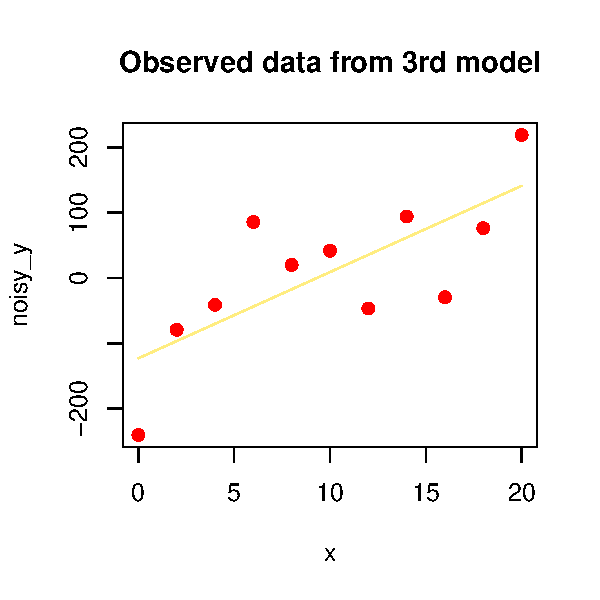
\includegraphics[height=35mm]{deg1}}
\only<3>{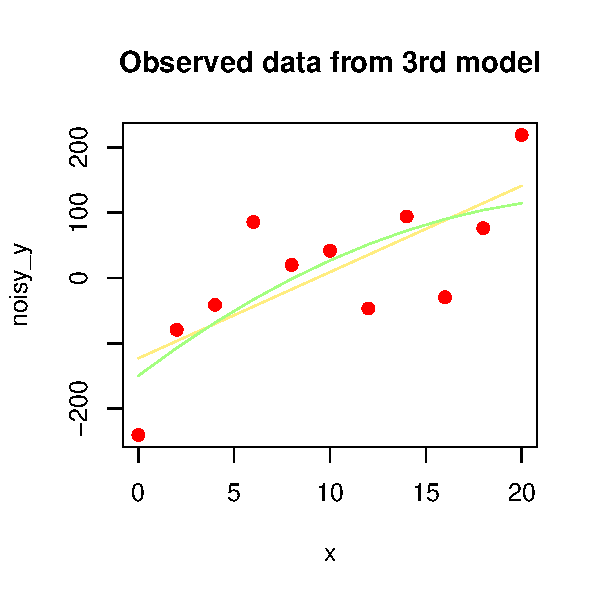
\includegraphics[height=35mm]{deg2}}
\only<4>{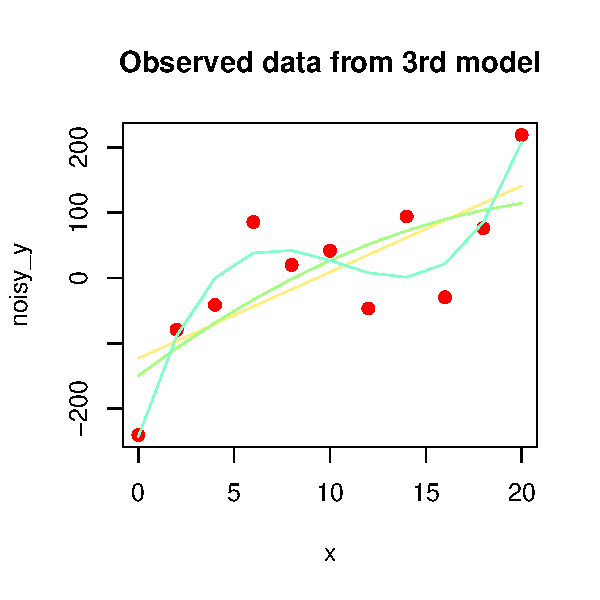
\includegraphics[height=35mm]{deg3}}
\only<5>{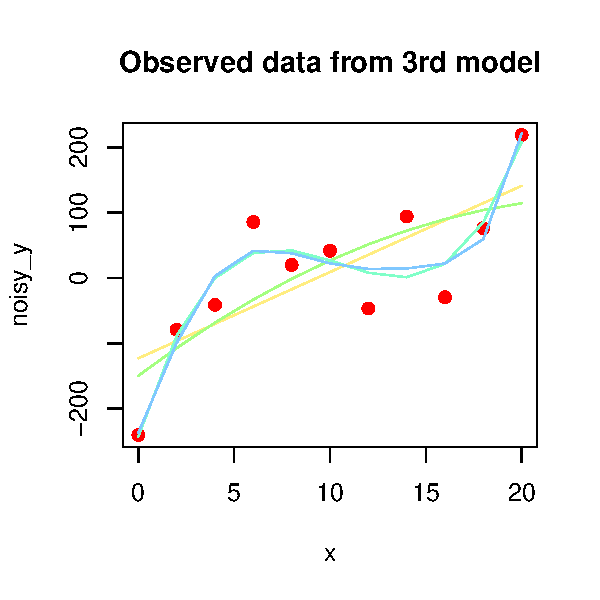
\includegraphics[height=35mm]{deg6}}
\only<6>{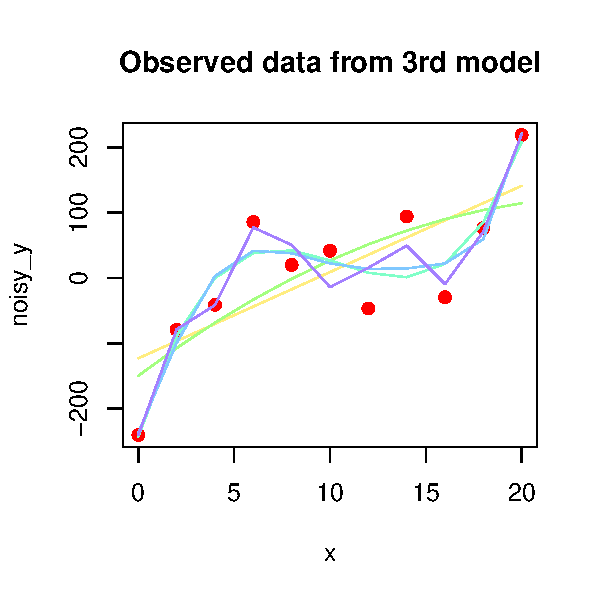
\includegraphics[height=35mm]{deg8}}
\only<7>{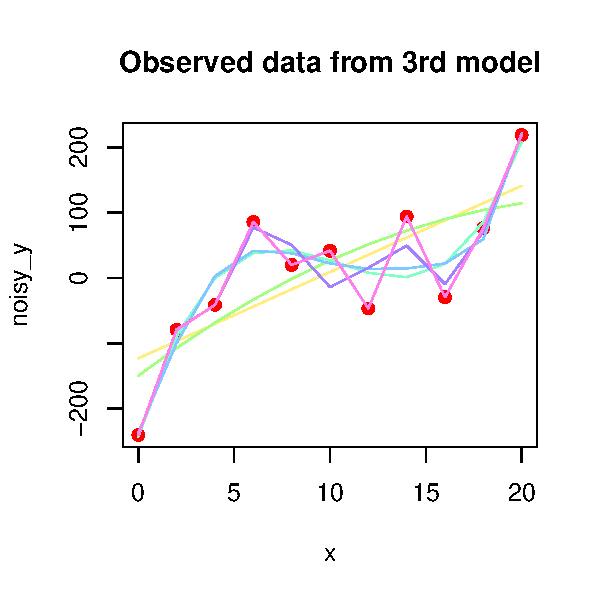
\includegraphics[height=35mm]{deg10}}
\end{center}
What is happening to our model as the degree increases?}
\only<8>{Overfitting can happen with linear regression too!
\begin{center}
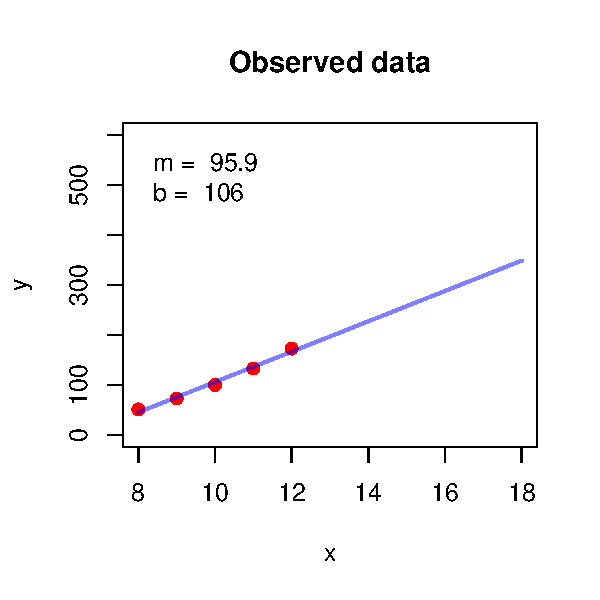
\includegraphics[height=40mm]{linfit1}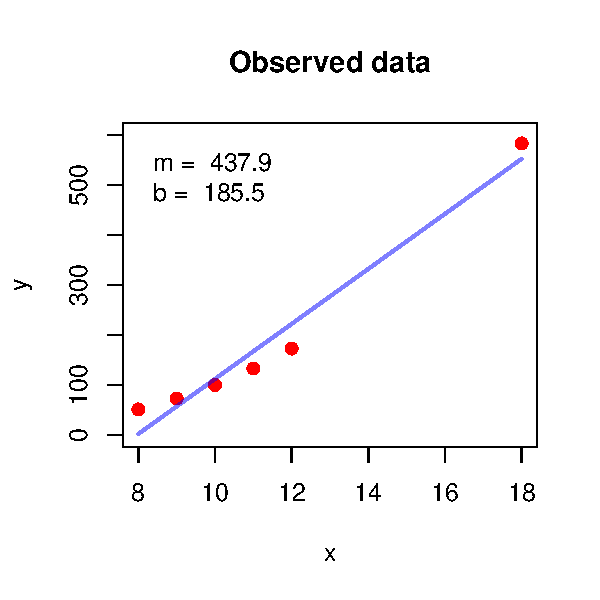
\includegraphics[height=40mm]{linfit2}
\end{center}
\vskip0.2cm
In multiple linear regression, what happens when we have $N$ number of observations and $N$ number of explanatory variables?
}
\only<9>{Overfitting happens when we learn parameters or rules that are too specific to the training set, so much that our model is not useful in explaining new data (we do great on train data but poorly on test).
\vskip0.4cm
Overfitting can happen when we have too few observations compared to the number of variables in our model with which we try to explain the observations.
\vskip0.4cm
We'll see that overfitting can be curbed by regularization and variable selection.
}
\end{frame}

\begin{frame}{Encoding Our Implicit Beliefs/Biases}
\only<1>{Before even seeing the California housing data, we already have a set of \textbf{beliefs} about the possible values for the parameters in our model, 
\begin{align}
P = mA + b + \epsilon.
\end{align}
\begin{enumerate}
\item $m$ can't be negative
\item $b$ can be negative, but will probably be positive
\item values of $m$ and $b$ can't be too large (to prevent overfitting)
\end{enumerate}
\vskip0.2cm
If we want the parameters we learn to reflect these beliefs, we must \emph{incorporate them into our model}.}
\only<2->{
We can translated these beliefs about the values of $m$ and $b$ into math
\vskip0.2cm
\begin{enumerate}
\item $m$ can't be negative and can't be too large
\begin{center}
\only<2>{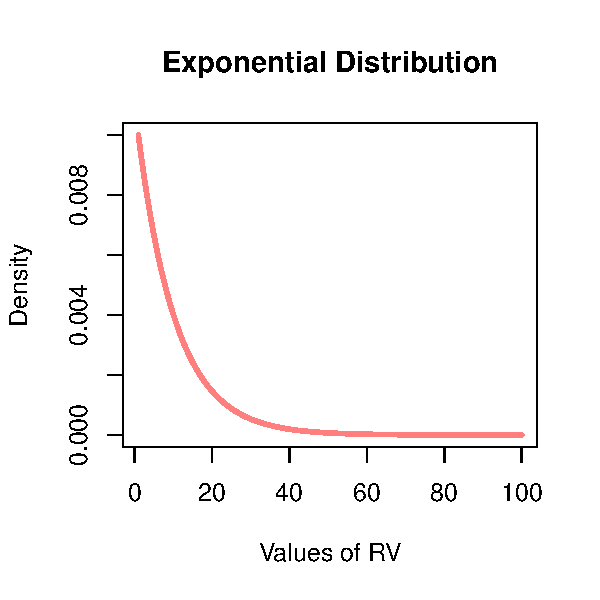
\includegraphics[height=30mm]{dist3}\\}
$m\sim \mathrm{Exp}(0.1), \quad p(m) = 0.1 e^{-0.1m}$
\end{center}

\only<3->{\item $b$ will probably be positive and can't be too large
\begin{center}
\only<3>{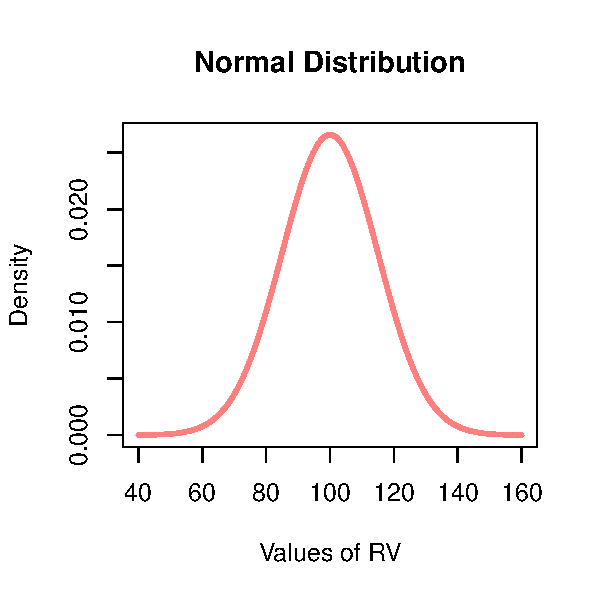
\includegraphics[height=30mm]{dist1}\\}
\only<3-4>{$b\sim \mathcal{N}(100, 15), \quad p(b) = \frac{1}{\sqrt{2\pi \cdot 15^2}} e^{-\frac{1}{2} \left( \frac{b - 100}{15}\right)^2}$}
\end{center}
}
\end{enumerate}
\only<4>{
\vskip0.2cm
The distributions encoding our \emph{prior beliefs} about the parameters $m$ and $b$ are called \textbf{priors}.}
}
\end{frame}

\begin{frame}{Bayesian Statistical Models}
\vskip-0.4cm
A \textbf{Bayesian statistical model} is a statistical model that incorporates \emph{priors} beliefs about the parameters of the model.
\vskip0.2cm
\begin{block}{A Bayesian Price Model}
Recall our linear model for housing prices:
\begin{align*}
& P = mA + b + \mathrm{\epsilon}\\
& \begin{cases}
\epsilon \sim \mathcal{N}(\mu_1, \sigma_1)
\end{cases} &  (\text{Distribution of Noise}) \\
& \begin{cases}
b \sim  \mathcal{N}(\mu_2, \sigma_2)\\
m \sim \mathrm{Exp}(\lambda)
\end{cases} & (\text{Priors on Parameters}) 
\end{align*}
where we picked $\mu_1 = 0$, $\sigma_1 = 1$, $\mu_2 = 100$, $\sigma_2 = 15$, $\lambda = 0.1$.
\end{block}
\end{frame}

\begin{frame}{The Posterior Distribution}
\only<1>{Learning values for the parameters that takes into account the priors as well as the data is called \emph{Bayesian inference}. 
\vskip0.4cm
But just how do we learn while accounting for priors?}
\only<2>{\small
Consider the distribution of the model parameters \emph{given} the data and the model
\begin{align}
p(m, b | P, A, \epsilon);
\end{align}
this is called the \textbf{posterior distribution}. 
\vskip0.4cm
Using Baye's Theorem, we computed the posterior to be
\begin{align*}
p(m, b | P, A, \epsilon) &= \frac{p(P | m, A, b, \epsilon)p(m)p(b)}{p(P)} \\
&\propto \underbrace{p(P | m, A, b, \epsilon)}_{Likelihood}\underbrace{p(m)p(b)}_{Priors}\\
\end{align*}
}
\end{frame}

\begin{frame}{Bayesian Inference}\footnotesize
\vskip-0.4cm
Working with the \emph{posterior distribution} accounts for prior beliefs.
\begin{enumerate}
\item (Non-Bayesian) Learn parameters, $m$ and $b$, to maximize the likelihood, i.e. the `probability' of \emph{data given the parameters},
\[
m^{MLE}, b^{MLE} = \underset{m, b}{\mathrm{argmax}}\; p(P | m, A, b, \epsilon)
\]
$m^{MLE}, b^{MLE}$ are called \emph{maximum likelihood estimates}. 
\vskip0.2cm
\item (Bayesian) Learn parameters, $m$ and $b$, to maximize the posterior, i.e. the `probability' of \emph{parameters given the data and the priors}, 
\[
m^{MAP}, b^{MAP} = \underset{m, b}{\mathrm{argmax}}\;  p(m, b | P, A, \epsilon)\propto \underbrace{p(P | m, A, b, \epsilon)}_{Likelihood}\underbrace{p(m)p(b)}_{Priors}
\]
$m^{MAP}, b^{MAP} $ are called \textbf{maximum a posteriori estimates}. 
\end{enumerate}
\end{frame}

\begin{frame}{Priors and Regularization}
\vskip-0.4cm
\only<1>{Again, maximizing the posterior distribution can be written as minimizing a loss function that penalizes certain kinds of model parameters.
\vskip0.2cm
\begin{enumerate}
\item ($\ell_1$ regularization) If the parameters have \emph{Laplace priors} then 
\[
m^{MAP}, b^{MAP} = \underset{a_1, a_0}{\mathrm{argmin}}\sum_{i=1}^n \left| y_i - (a_1x_i + a_0)\right|^2 + (|a_1| + |a_0|)
\]
\item ($\ell_2$ regularization) If the parameters have \emph{normal priors} then 
\[
m^{MAP}, b^{MAP} = \underset{a_1, a_0}{\mathrm{argmin}}\sum_{i=1}^n \left| y_i - (a_1x_i + a_0)\right|^2 + \sqrt{a_1^2 + a_0^2}
\]
\end{enumerate}
}
\only<2>{
\begin{enumerate}
\item ($\ell_1$ regularization) With $\ell_1$ regularization,
\[
m^{MAP}, b^{MAP} = \underset{a_1, a_0}{\mathrm{argmin}}\sum_{i=1}^n \left| y_i - (a_1x_i + a_0)\right|^2 + (|a_1| + |a_0|)
\] 
we are biased towards models with fewer predictors (fewer non-zero parameters). 
\vskip0.2cm
\item ($\ell_2$ regularization) With $\ell_2$ regularization, 
\[
m^{MAP}, b^{MAP} = \underset{a_1, a_0}{\mathrm{argmin}}\sum_{i=1}^n \left| y_i - (a_1x_i + a_0)\right|^2 + \sqrt{a_1^2 + a_0^2}
\]
we are biased towards models with smaller parameters. 
\end{enumerate}
}
\end{frame}

%%%%%%%%%%%%%%%%%%%%%%%%%%%%%%%%%%%%%%%%%%%%%%%%%%%%%%%%%%%%%%%%%%%%%%%%%%%%%%
\section{Application: Land Use Regression}

\begin{frame}{Overview of Air Quality Models}
\vskip-0.4cm
\emph{Air quality models} characterizes the distribution of concentrations of atmospheric pollutants over time and or space. There are two major categories of air quality models:
\vskip0.2cm
\begin{enumerate}
\item \textbf{Deterministic:} these are typically diffusion models that model the movement of atmospheric particles systems, incorporating physical forces and chemical processes
\vskip0.2cm
\item \textbf{Statistical:} these are models whose corrlate the concentration level of the pollutant with a set of spatio-temporal predicators, incorporating random noise.
\end{enumerate}
\vskip0.2cm
\emph{Land Use Regression model} is an example of a statistical air quality model.
\end{frame}

\begin{frame}{Land Use Regression Models: Spatial}
\vskip-0.4cm
\only<1>{
\textbf{Motivation:} Typically monitoring stations are few in number and statically located. There is not enough observed data to understand fine-grained variation of pollution across a region. 
\vskip0.2cm
Given a set of average readings at $n$ number of sites, $\{p_1, \ldots, p_n\}$, we fit a linear model correlating the land use characteristic, $\{L_1, \ldots, L_J\}$, around each site with the reading at the site:
\[
p = a_0 + \sum_{i=1}^J a_i L_i \quad\quad (\textbf{Land Use Regression Model})
\]
Typically, we grid the region of interest and extract the same set of land use characteristics $\{L_1, \ldots, L_J\}$ for each grid cell. }
\only<2>{
\vskip0.6cm
\textbf{Question:} How to we use the model 
\[
p = a_0 + \sum_{i=1}^J a_i L_i \quad\quad (\textbf{Land Use Regression Model})
\]
fitted on the readings from the stations, $\{p_1, \ldots, p_n\}$, to fill in the missing observations in other areas?
}
\end{frame}

\end{document}
